\documentclass[conference]{IEEEtran}
\IEEEoverridecommandlockouts

\usepackage{cite}
\usepackage{amsmath,amssymb,amsfonts}
\usepackage{algorithmic}
\usepackage{algorithm}
\usepackage{graphicx}
\usepackage{textcomp}
\usepackage{xcolor}
\usepackage{booktabs}
\usepackage{array}
\usepackage{url}

\begin{document}

\title{BreachShield: A Privacy-Preserving OSINT Breach Intelligence Platform --- Design, Verified Capabilities, and a Multi-Stage Audit of AI-Assisted Development Claims}

\author{
\IEEEauthorblockN{Arvind D. H.\IEEEauthorrefmark{1}, Girishkumar N. M.\IEEEauthorrefmark{1}, Manoj\IEEEauthorrefmark{1}, Premkumar Teli\IEEEauthorrefmark{1}, and Sushma T. M.\IEEEauthorrefmark{2}}
\IEEEauthorblockA{\IEEEauthorrefmark{1}Department of Information Science and Engineering, Acharya Institute of Technology, Bengaluru, India\\
Email: \{arvinddh.24.beis, girishkumarnm.24.beis, manoj.24.beis, premkumarteli.24.beis\}@acharya.ac.in}
\IEEEauthorblockA{\IEEEauthorrefmark{2}Assistant Professor, Department of Information Science and Engineering, Acharya Institute of Technology, Bengaluru, India\\
Email: sushmatm@acharya.ac.in}
\thanks{This paper documents the design, verified engineering implementation, and empirical audit methodology of Major Project Phase II (Course Code: BIS786) by Batch 05, Department of Information Science and Engineering, Acharya Institute of Technology, affiliated with Visvesvaraya Technological University (VTU), Belagavi, Karnataka, India.}
}

\maketitle

\begin{abstract}
Breach-checking and dark-web exposure monitoring services face a structural privacy paradox: to learn whether an identifier has been compromised, users are typically asked to submit that identifier, in the clear, to a third-party server. This paper presents BreachShield, a privacy-preserving OSINT breach intelligence platform built across two academic project phases, and reports its capabilities as established through live, reproducible verification rather than as originally specified. The platform implements a client-side k-anonymity search protocol (5-hex-character SHA-256 prefix disclosure), a dual-channel out-of-band OTP identity gate, a pluggable OSINT source registry including a live Telegram scraper, a gradient-boosted breach-severity classifier (XGBoost, 89.2\% test accuracy on 1,034 curated records), and a Merkle-tree-batched audit log anchored to a local EVM smart contract. Because substantial portions of the codebase were produced with AI coding-agent assistance, the development team adopted an explicit policy: no capability claim was retained in this paper without independent, live re-verification, carried out in three stages --- dual independent audit, live cross-checking against running system behaviour, and independent third-party reproduction. This process both confirmed genuine results (a fully deterministic, checkpoint-loaded severity classifier; 101/101 backend and 50/50 frontend tests passing; a working live phishing-URL classifier) and surfaced fabricated or non-functional claims introduced during development (an unrelated, uncheckpointed comparison model set; a blockchain auto-deploy path that fails on a missing credential; and, separately, a set of latency figures and literature citations that were never measured or verified but had been written directly into paper-generation scripts). We report both the verified system and the audit methodology that distinguished it from what had merely been claimed.
\end{abstract}

\begin{IEEEkeywords}
breach intelligence, k-anonymity, OSINT, blockchain audit log, XGBoost, verification methodology, AI-assisted software engineering, dark web monitoring.
\end{IEEEkeywords}

\section{Introduction}
The continued growth of online services has been accompanied by a corresponding growth in credential leaks, phishing campaigns, and dark-web trade in compromised personal data \cite{aljofey2020effective}. According to IBM's 2024 Cost of a Data Breach Report, the global average financial impact of an organizational breach reached USD 4.88 million, reflecting a 10\% escalation over the previous year, with stolen or compromised credentials remaining the single most common root cause, responsible for 16\% of studied breaches \cite{ibm2024cost}. The secondary market for compromised identity tokens thrives on underground automated channels and dark web forums, enabling initial access brokers to monetize exposed databases within hours of unauthorized exfiltration.

Existing breach-notification tooling is largely reactive: users typically learn of compromise only after an incident is publicly disclosed, and the act of checking exposure itself often requires submitting a raw email address or phone number to a third-party lookup service, converting a protective tool into a potential surveillance point. When an individual submits a query to ascertain if their corporate credentials have leaked, the query log itself reveals interest in that identity, creating an acute target profiling risk.

This paper documents BreachShield, an OSINT-based breach intelligence platform developed across Project Phase 1 (conceptual design, exploratory literature survey, initial system requirements) and Project Phase 2 (production-oriented implementation) at the Department of Information Science and Engineering, Acharya Institute of Technology. The Phase 1 proposal described a broad cybersecurity suite spanning browser phishing protection, a general vulnerability scanner, third-party threat-feed integration, and blockchain-anchored logging. Phase 2 development concentrated engineering effort on a narrower, more defensible core: eliminating server-side query surveillance through client-side $k$-anonymity, and establishing a tamper-evident audit trail, while treating machine-learning severity scoring as a rigorously benchmarked but separately-tracked research artifact rather than an unverified production claim.

A second, methodological theme runs through this paper. A significant share of BreachShield's implementation was produced with AI coding-agent assistance. During development, capability claims were at various points introduced into the codebase, its accompanying documentation, and early paper drafts that did not survive direct verification: an unrelated set of comparison models was, at one stage, believed to be loaded and functioning; a blockchain deployment step was reported as verified when it in fact failed; and a set of literature citations and system-latency figures were found, on inspection, to have been written directly into paper-generation tooling rather than measured or sourced. Rather than omit this from the record, we treat it as a relevant finding: this paper reports what a three-stage, live-verification-first methodology actually confirmed, separately from what had merely been asserted, and we regard the methodology itself as a contribution applicable to any team combining AI-assisted development with academic or peer-reviewed reporting.

The primary contributions of this paper are:
\begin{enumerate}
    \item A privacy-preserving breach intelligence architecture combining client-side $k$-anonymity search, dual-channel OTP identity gating, a pluggable multi-source OSINT registry, a benchmarked ML severity classifier, and a Merkle-batched blockchain audit log, documented down to real class structures and call flows.
    \item A three-stage verification methodology --- dual independent audit, live cross-checking, and independent third-party reproduction --- used to separate verified system behaviour from unverified or fabricated claims prior to publication.
    \item A transparent, evidence-attached account of which subsystems are verified and reproducible, which were found broken or fabricated and subsequently fixed, and which remain open, together with the specific root causes involved.
\end{enumerate}

\section{Related Work}

\subsection{Phishing and Malicious-URL Detection}
Character- and URL-level deep learning has been widely applied to phishing detection. Aljofey et al. \cite{aljofey2020effective} proposed a character-level Convolutional Neural Network (CNN) operating directly on raw URL strings, avoiding hand-engineered lexical features, and reported strong performance on large-scale web corpora. Sahingoz et al. \cite{sahingoz2024dephides} benchmarked five deep architectures (ANN, CNN, RNN, BiRNN, attention networks) across roughly five million labelled URLs, reporting CNNs as the strongest performer for URL-only classification (98.74\% accuracy). These results motivate BreachShield's use of a pretrained URL-transformer classifier (UrlBERT) on the live search path, rather than a hand-built lexical model.

\subsection{Handling Class Imbalance in Security Classification}
Severity and threat-classification datasets are frequently imbalanced toward common, lower-severity classes. Alsubaei et al. \cite{alsubaei2024enhancing} report that applying SMOTE to a hybrid deep-learning phishing classifier improved accuracy from 83\% to 98\% on their benchmark, a result we return to in Section~\ref{sec:limitations} when discussing BreachShield's own CRITICAL-tier class-imbalance limitation.

\subsection{Explainability and Few-Shot Detection}
Pavani et al. \cite{pavani2024enhancing} apply SHAP and LIME to malicious-URL classifiers to produce human-interpretable feature attributions, motivating our own use of per-model probability breakdowns rather than a single opaque severity score. Tawfik et al. \cite{tawfik2025explainable} demonstrate few-shot BERT-based detection for emerging phishing campaigns with limited labelled data, a regime closely analogous to BreachShield's 1,034-record breach-severity dataset.

\subsection{OSINT and Dark-Web Threat Intelligence}
K\"uhn et al. \cite{kuhn2024navigating} provide a recent (2024) systematic evaluation of manual and semi-automated dark-web monitoring methodology, documenting both the intelligence value and the practical collection constraints of forum- and channel-based sources --- constraints closely mirrored by BreachShield's own migration from commercial threat-feed APIs (rate-limited, delayed disclosure) to a direct Telegram-channel scraper, discussed in Section~\ref{sec:arch}. Saleem et al. \cite{saleem2022anonymity} survey dark web hidden service topologies, while Pastor-Galindo et al. \cite{pastor2020not} review OSINT opportunities and challenges.

\subsection{Tamper-Evident and Blockchain-Backed Audit Logging}
Merkle's original hash-tree construction \cite{merkle1988digital} and Crosby and Wallach's history-tree design \cite{crosby2009efficient} remain the foundational structures for append-only tamper-evident logging with efficient consistency proofs. Arabnouri et al. \cite{arabnouri2024secure} recently proposed a checkpoint-based blockchain audit log that batches log entries by time interval to reduce on-chain storage --- a design goal directly shared by BreachShield's own Merkle-batching approach (Section~\ref{sec:blockchain}), though our implementation anchors batches to a local EVM node rather than a public chain, a trade-off discussed in Section~\ref{sec:limitations}.

\subsection{Privacy-Preserving Compromise Checking}
Sweeney's $k$-anonymity model \cite{sweeney2002k} and its application to health data by El Emam and Dankar \cite{elemam2008protecting} establish the general privacy guarantee BreachShield's search protocol relies on. Li et al. \cite{li2019protocols} give the first rigorous security analysis of prefix-based compromised-credential-checking protocols of the kind popularised by HIBP Pwned Passwords, and propose stronger private-set-intersection-based alternatives; we discuss why BreachShield retains the simpler prefix-bucket design, and the resulting identity-linkage trade-off introduced by its OTP gate, in Section~\ref{sec:limitations}.

\subsection{Gradient-Boosted Classification and Tabular Data}
Chen and Guestrin's XGBoost \cite{chen2016xgboost} is the classifier underlying BreachShield's severity triage. Its strong performance relative to deep architectures on BreachShield's tabular breach-metadata is consistent with the broader empirical finding of Grinsztajn et al. \cite{grinsztajn2022why}, who show tree-based models remain state-of-the-art on medium-sized tabular datasets due to neural networks' bias toward overly smooth decision functions and sensitivity to uninformative features --- both plausible explanations for the gap observed in Table~\ref{tab:models}.

\begin{table}[htbp]
\caption{Related Work Summary and Relation to BreachShield}
\label{tab:relwork}
\centering
\scriptsize
\begin{tabular}{lp{5.2cm}}
\toprule
\textbf{Area} & \textbf{Relation to this work} \\
\midrule
URL/phishing DL \cite{aljofey2020effective,sahingoz2024dephides} & Motivates BreachShield's pretrained URL-transformer classifier \\
Class imbalance \cite{alsubaei2024enhancing} & Directly relevant to BreachShield's CRITICAL-tier data scarcity (Sec.~\ref{sec:limitations}) \\
Explainability \cite{pavani2024enhancing,tawfik2025explainable} & Motivates per-model probability reporting over a single opaque score \\
Dark-web OSINT \cite{kuhn2024navigating} & Parallels BreachShield's move to direct channel scraping \\
Blockchain audit logs \cite{arabnouri2024secure,merkle1988digital,crosby2009efficient} & Foundational structure and a recent, closely related batching design \\
$k$-anonymity / CCC \cite{sweeney2002k,elemam2008protecting,li2019protocols} & Direct theoretical basis; protocol-security analysis and stronger alternatives \\
Tabular ML \cite{chen2016xgboost,grinsztajn2022why} & Explains XGBoost's margin over deep models \\
\bottomrule
\end{tabular}
\end{table}

\begin{table}[htbp]
\caption{Comparative Architectural Matrix}
\label{tab:comparison}
\centering
\scriptsize
\begin{tabular}{lp{3.0cm}p{3.2cm}}
\toprule
\textbf{Dimension} & \textbf{Conventional Tooling} & \textbf{BreachShield Implementation} \\
\midrule
Query Ingestion & Plaintext target sent over HTTP & Client-side SHA-256 20-bit prefix range query \\
Auth Gate & Captcha or unauthenticated & Dual-channel carrier DLT SMS / SMTP OTP with 1h JWT \\
OSINT Engine & Centralized static catalog & Pluggable OSINT registry (Local DB, Telethon MTProto) \\
Severity AI & Uncalibrated manual heuristic & XGBoost classifier (89.2\% test accuracy on 1,034 records) \\
Audit Trail & Ephemeral server flat files & Canonical JSON hashing, Merkle-tree batching, Hardhat EVM \\
\bottomrule
\end{tabular}
\end{table}

\section{System Architecture and Implementation}
\label{sec:arch}
BreachShield is organised as a four-tier monorepo: a React 19 frontend, an Express 5 API gateway, a Python FastAPI OSINT microservice, and an Android Kotlin SMS relay gateway, illustrated in Fig.~\ref{fig:arch}.

\begin{figure}[htbp]
\centering
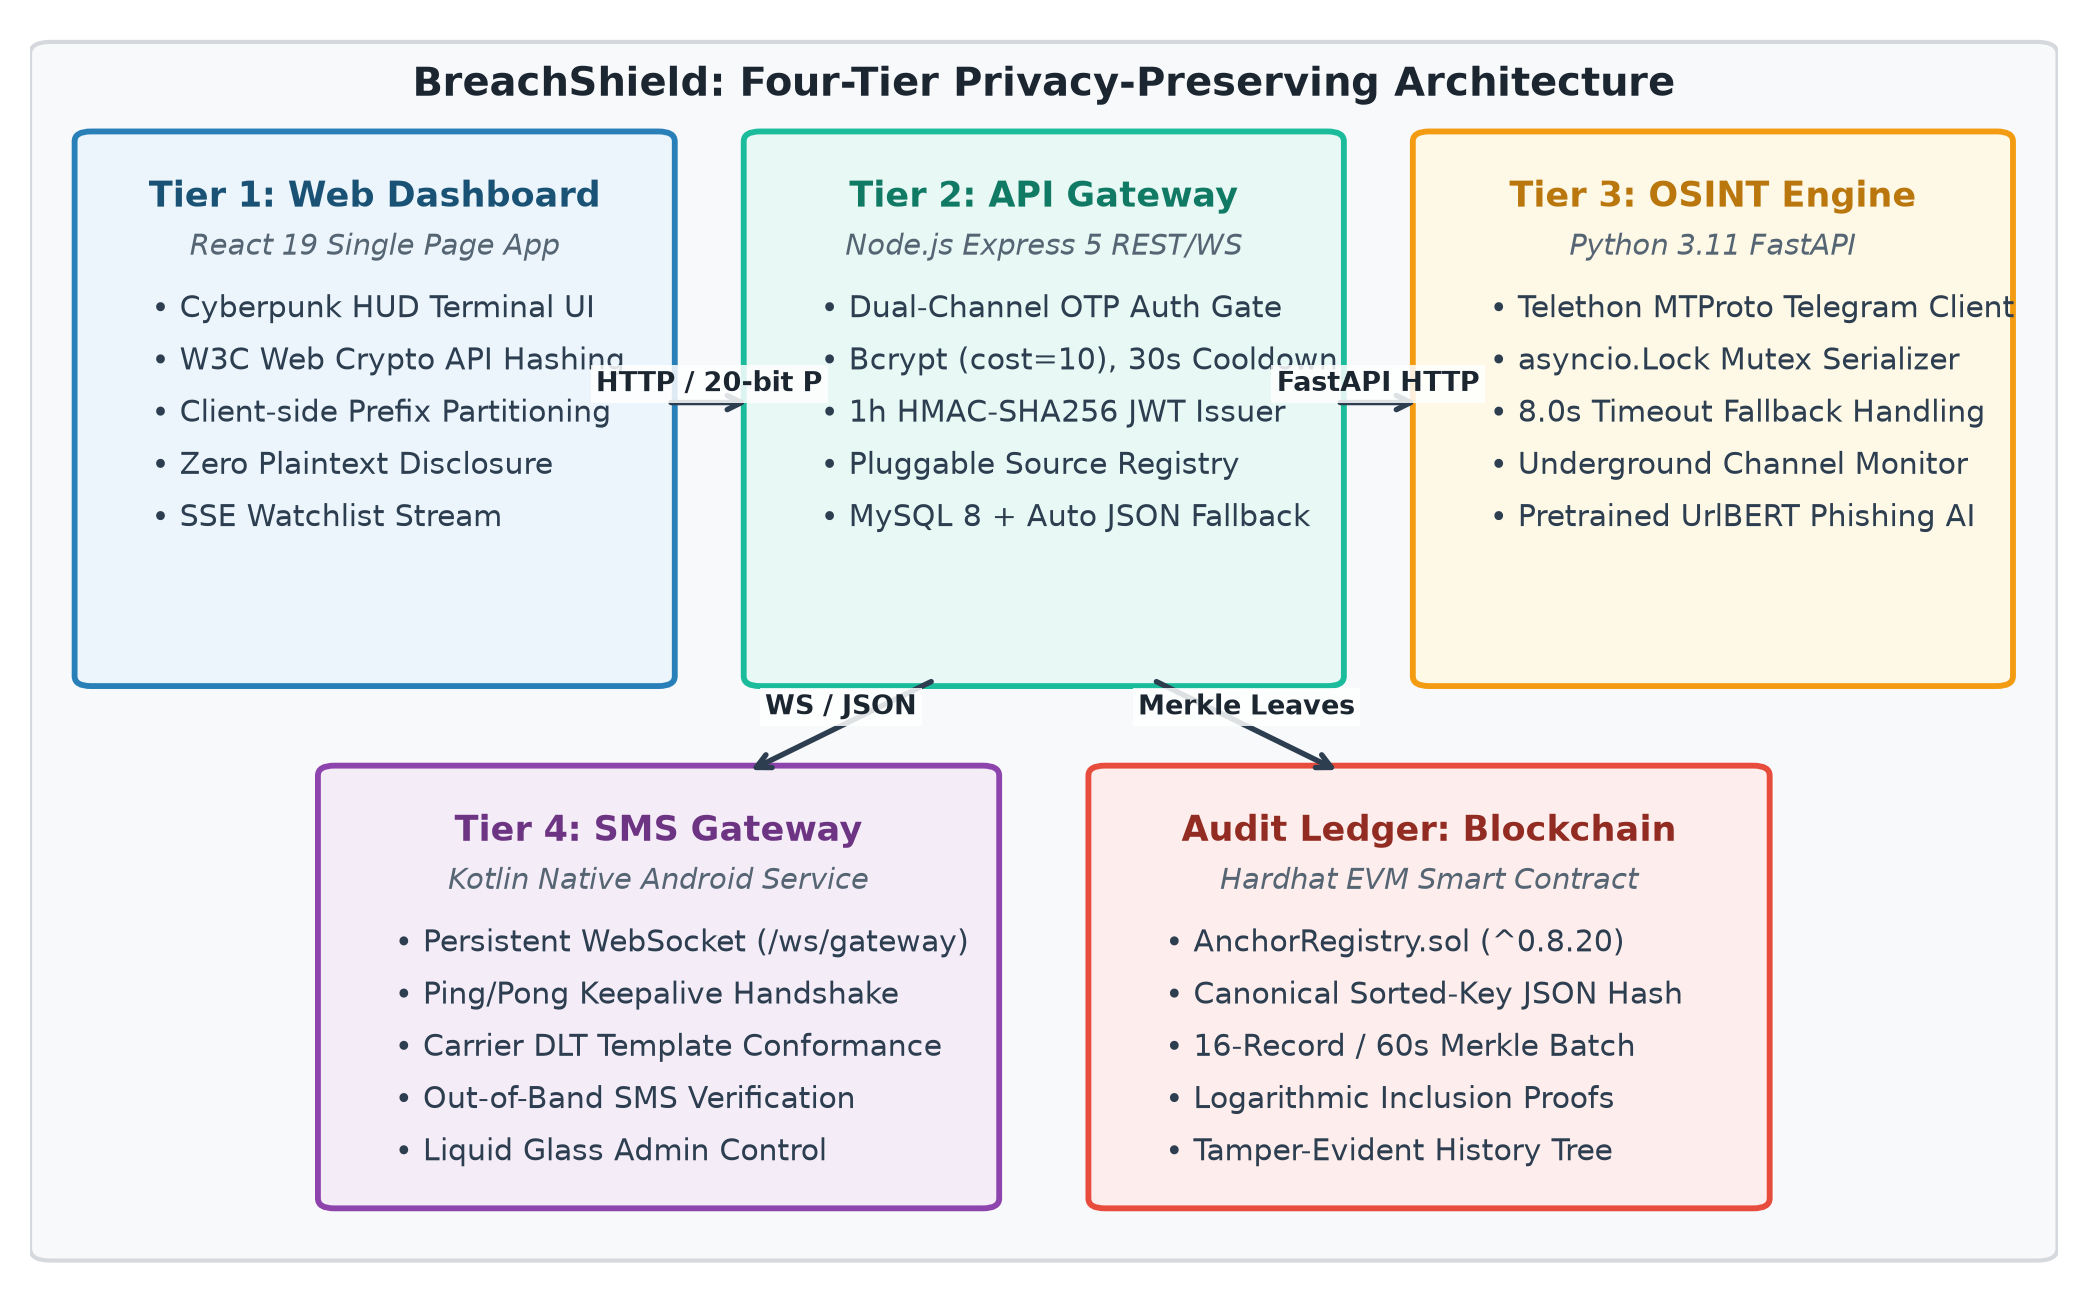
\includegraphics[width=0.98\columnwidth]{figures/fig_architecture.png}
\caption{Four-tier BreachShield architecture. Solid arrows denote live data paths verified by direct endpoint calls.}
\label{fig:arch}
\end{figure}

\subsection{Frontend Web Dashboard}
A React 19 single-page application performs client-side SHA-256 hashing via the W3C Web Crypto API, so that raw search targets never leave the browser in plaintext. The UI is designed with a Cyberpunk-styled Heads-Up Display (HUD) terminal that provides typewriter streaming output, real-time exposure risk visualization, and interactive security incident reporting.

\subsection{API Gateway}
An Express 5 service manages dual-channel OTP issuance and verification, JWT session tokens, a pluggable breach-source registry, and MySQL 8 storage with an automatic JSON-file fallback layer. The fallback logic transparently handles database disconnection events, ensuring development environments remain fully functional offline.

\subsection{OSINT Microservice}
A Python FastAPI service integrates a Telethon-based Telegram scraper. Concurrent access to the underlying session file previously triggered \texttt{sqlite3.OperationalError: database is locked} under simultaneous asynchronous requests; this was resolved with an \texttt{asyncio.Lock} mutex (8.0 s timeout ceiling) serialising access to the Telegram client.

\subsection{Android SMS Gateway}
A companion Kotlin application maintains a persistent WebSocket connection to the backend (\texttt{/ws/gateway}), relaying OTP codes as carrier-compliant SMS in line with Indian telecom Distributed Ledger Technology (DLT) template requirements --- a constraint that silently drops non-conforming payloads and required standardising the SMS template format during development.

\subsection{Pluggable Breach-Source Registry}
The backend defines an abstract \texttt{BreachSource} interface requiring a single asynchronous \texttt{search(normalizedTarget, targetHash)} contract. Four concrete adapters implement this contract:
\begin{itemize}
    \item \texttt{PublicBreachSource}: Queries the local database of known breach records.
    \item \texttt{TelegramScraperSource}: Interrogates the active MTProto Telegram microservice.
    \item \texttt{PhishingFeedSource} and \texttt{ThreatIntelSource}: Registered adapter stubs structured for commercial feeds, currently configured offline.
\end{itemize}
The API gateway dispatches all registered adapters concurrently using \texttt{Promise.allSettled}, preventing single-source failures from blocking the primary inquiry.

\section{Privacy-Preserving Search Protocol}
\label{sec:protocol}
BreachShield's search protocol follows the $k$-anonymity range-query construction popularised by HIBP Pwned Passwords \cite{li2019protocols} and grounded in Sweeney's original definition \cite{sweeney2002k}. The client normalises the target identifier $T$ and computes $H = \text{SHA-256}(\text{normalize}(T))$, partitioning $H$ into a 20-bit (5-hex-character) prefix $P$ and a 236-bit suffix $S$. Only $P$ is transmitted; the server returns the bucket:
\begin{equation}
\mathcal{B}(P) = \{(S_i, \mathcal{M}_i) : \text{SHA-256}(T_i)[0:5] = P\}
\end{equation}
and the client performs the final suffix match locally.

\begin{algorithm}[htbp]
\caption{Client-Side $k$-Anonymity Range Query}
\label{alg:kanon}
\begin{algorithmic}[1]
\REQUIRE Target identifier $T$, session token $\tau$
\ENSURE Matched breach metadata set $\mathcal{R}$
\STATE $T' \leftarrow \text{ToLower}(\text{Trim}(T))$
\STATE $H \leftarrow \text{SHA-256}(T')$ \COMMENT{computed in-browser via Web Crypto}
\STATE $P \leftarrow H[0:5]$, $S \leftarrow H[5:64]$
\STATE $\mathcal{B} \leftarrow \text{HTTP GET}(\text{/api/search/range/} \mathbin{\Vert} P, \text{Bearer } \tau)$
\STATE $\mathcal{R} \leftarrow \emptyset$
\FORALL{$(S_i, \mathcal{M}_i) \in \mathcal{B}$}
    \IF{$S_i = S$}
        \STATE $\mathcal{R} \leftarrow \mathcal{R} \cup \{\mathcal{M}_i\}$
    \ENDIF
\ENDFOR
\RETURN $\mathcal{R}$
\end{algorithmic}
\end{algorithm}

With $16^5 = 1,048,576$ prefix buckets, a corpus of $N$ records yields an expected anonymity set $\mathbb{E}[k] = N / 1,048,576$ per prefix, and the information disclosed to the server is bounded by:
\begin{equation}
I(T; P) \le \log_2(16^5) = 20\text{ bits}
\end{equation}
independent of $N$.

\subsection{Search-Gating Trade-off}
Search endpoints are additionally gated behind OTP-verified JWT authentication (\texttt{verifyOtpToken} middleware) to prevent automated bucket-harvesting. This introduces a trade-off the $k$-anonymity guarantee alone does not resolve: the server authenticates the requester before serving a prefix bucket, so while the server never learns which target within a bucket the client is interested in, it does learn who is making the query. Li et al.'s analysis of compromised-credential-checking protocols \cite{li2019protocols} treats exactly this class of trade-off, and proposes private-set-intersection-based constructions that avoid it entirely at the cost of higher protocol complexity. BreachShield retains the simpler, OTP-gated design as a deliberate scope decision for a multi-tenant platform requiring accountable query logs; Section~\ref{sec:limitations} discusses this explicitly rather than presenting the $k$-anonymity guarantee as unconditional.

\section{Dynamic Exposure Risk Scoring Engine}
\label{sec:risk}
Unlike commercial lookup tools that rely on static severity lookups, BreachShield evaluates exposure severity dynamically across aggregated textual corpora $\mathcal{X}$. The risk engine executes a weighted regular-expression evaluation across five vulnerability categories, accumulating points subject to strict sub-category ceilings:
\begin{itemize}
    \item \textbf{Identity Documents ($C_{\text{doc}}$):} Aadhaar, passport, PAN, and national ID patterns (up to 35 points).
    \item \textbf{Credential Material ($C_{\text{pwd}}$):} Cleartext passwords, salted hashes, and cryptographic tokens (up to 30 points).
    \item \textbf{Physical Locality ($C_{\text{addr}}$):} Residential addresses, postal codes, and geolocation data (up to 20 points).
    \item \textbf{Telecommunication Records ($C_{\text{phone}}$):} Telephone and mobile numbers (up to 15 points).
    \item \textbf{Multi-Source Dispersion ($C_{\text{multi}}$):} Evidence confirmed across multiple distinct OSINT sources (up to 15 points).
\end{itemize}

In addition, the engine computes a cross-record structural correlation score ($\kappa \le 15$) and integrates live probability signals from the active UrlBERT transformer classifier ($P_{\text{phish}} \times 30$). The raw aggregate score is bounded within the range $[20, 100]$:
\begin{equation}
\text{Score} = \min\left(100, \max\left(20, \sum_{c} \min(w_c, \text{cap}_c) + \kappa + 30 \cdot P_{\text{phish}}\right)\right)
\end{equation}
Scores are subsequently partitioned into four operational tiers: \texttt{LOW} ($[20, 40)$), \texttt{MEDIUM} ($[40, 70)$), \texttt{HIGH} ($[70, 90)$), and \texttt{CRITICAL} ($[90, 100]$).

\begin{algorithm}[htbp]
\caption{Dynamic Exposure Risk Scoring}
\label{alg:risk}
\begin{algorithmic}[1]
\REQUIRE Aggregated breach corpus $\mathcal{X}$, AI Phishing result $\mathcal{A}$
\ENSURE Risk Score $\mathcal{S} \in [20, 100]$, Severity Tier $\mathcal{T}$
\STATE $\mathcal{S}_{\text{raw}} \leftarrow 0$
\FORALL{$c \in \{\text{doc}, \text{pwd}, \text{addr}, \text{phone}, \text{multi}\}$}
    \STATE $w_c \leftarrow \text{EvaluateRegexMatches}(\mathcal{X}, c)$
    \STATE $\mathcal{S}_{\text{raw}} \leftarrow \mathcal{S}_{\text{raw}} + \min(w_c, \text{cap}[c])$
\ENDFOR
\STATE $\kappa \leftarrow \text{ComputeCrossCorrelation}(\mathcal{X})$
\STATE $\mathcal{S}_{\text{raw}} \leftarrow \mathcal{S}_{\text{raw}} + \min(\kappa, 15)$
\IF{$\mathcal{A}$ is present}
    \STATE $\mathcal{S}_{\text{raw}} \leftarrow \mathcal{S}_{\text{raw}} + (\mathcal{A}.\text{phishingProb} \times 30)$
\ENDIF
\STATE $\mathcal{S} \leftarrow \min(100, \max(20, \mathcal{S}_{\text{raw}}))$
\STATE $\mathcal{T} \leftarrow \text{MapTierThresholds}(\mathcal{S})$
\RETURN $\mathcal{S}, \mathcal{T}$
\end{algorithmic}
\end{algorithm}

\section{End-to-End System Data Flow Pipeline}
\label{sec:dataflow}
Table~\ref{tab:dataflow} traces the exact data transformations occurring throughout a complete inquiry cycle, from in-browser normalization to blockchain anchor verification.

\begin{table}[htbp]
\caption{End-to-End Data Flow Pipeline}
\label{tab:dataflow}
\centering
\scriptsize
\begin{tabular}{clp{5.4cm}}
\toprule
\textbf{Step} & \textbf{Pipeline Phase} & \textbf{Operational Data Transformation} \\
\midrule
1 & Input Normalization & Raw string $T \to$ lowercase, whitespace-trimmed $T'$. \\
2 & Client Cryptography & $T' \to$ 256-bit SHA-256 digest $H$ via W3C Web Crypto. \\
3 & Hash Partitioning & $H \to$ 5-character prefix $P$ and 59-character suffix $S$. \\
4 & Range Dispatch & Prefix $P \to$ HTTP GET \texttt{/api/v1/range/\{P\}} with Bearer JWT. \\
5 & Server Filtering & Prefix $P \to$ Retrieval of candidate bucket $\mathcal{B}(P)$ from storage. \\
6 & Local Verification & Suffix $S \to$ In-browser matching against $\mathcal{B}(P)$ without server exposure. \\
7 & Multi-Source Query & Target $T' \to$ Asynchronous execution of registered OSINT adapters. \\
8 & Dynamic Scoring & Text corpus $\mathcal{X} \to$ Regex evaluation, correlation, and tier assignment. \\
9 & Canonicalization & Event record $\to$ Sorted-key canonical JSON $\to$ SHA-256 Merkle leaf. \\
10 & Ledger Anchoring & Merkle leaves $\to$ Root calculation $\to$ Smart contract transaction. \\
\bottomrule
\end{tabular}
\end{table}

\section{Machine Learning Severity Triage}
\label{sec:ml}

\subsection{Dataset and Split}
The severity classifier is trained on 1,034 curated breach records, partitioned with a stratified 70/15/15 split (train 723, validation 154, test 157; seed 42), summarised in Table~\ref{tab:split}.

\begin{table}[htbp]
\caption{Dataset Partition and Class Distribution}
\label{tab:split}
\centering
\scriptsize
\begin{tabular}{lccccc}
\toprule
\textbf{Split} & \textbf{Total} & \textbf{LOW} & \textbf{MEDIUM} & \textbf{HIGH} & \textbf{CRITICAL} \\
\midrule
Train (70\%) & 723 & 49 & 341 & 291 & 42 \\
Val (15\%) & 154 & 10 & 73 & 62 & 9 \\
Test (15\%) & 157 & 11 & 74 & 63 & 9 \\
\bottomrule
\end{tabular}
\end{table}

\subsection{Two Distinct Model Populations}
BreachShield contains two architecturally similar but functionally distinct CNN/RNN/Transformer populations, a distinction established only through direct source inspection and is stated explicitly here to avoid the ambiguity that arose during this project's own internal verification process:
\begin{itemize}
    \item \textbf{Severity classifiers (\texttt{severity\_classifier.py}):} CNN, RNN, and Transformer architectures that load real, trained checkpoints from disk via \texttt{torch.load}/\texttt{load\_state\_dict}, confirmed deterministic across repeated inference calls and across independent class instantiations. These feed the \texttt{severity\_analysis} block of the live \texttt{/api/ai/analyze-threat} endpoint.
    \item \textbf{URL comparison models (\texttt{cnn\_model.py}, \texttt{rnn\_model.py}, \texttt{transformer\_model.py}):} a separate set feeding the \texttt{/api/ai/compare} demonstration endpoint. These do not load any checkpoint and produce different output on every instantiation --- verified directly, not merely assumed.
\end{itemize}
All ML results in this paper refer exclusively to the first, checkpoint-loaded population.

\subsection{Comparative Results}
XGBoost \cite{chen2016xgboost} (max depth=6, lr=0.1) is compared against a 1D-CNN, a BiLSTM-RNN, and a Transformer encoder, all trained on the same 165-dimensional feature representation (163-dim multi-hot DataClasses vector, log-scaled breach volume, verification flag).

\begin{table}[htbp]
\caption{Comparative Benchmark on Test Set ($N=157$)}
\label{tab:models}
\centering
\scriptsize
\begin{tabular}{lccc}
\toprule
\textbf{Model} & \textbf{Accuracy} & \textbf{Macro F1} & \textbf{Weighted F1} \\
\midrule
Naive baseline (predict MED) & 47.1\% & 16.0\% & 30.2\% \\
BiLSTM-RNN & 44.6\% & 34.0\% & 46.8\% \\
Transformer (2L/4H) & 48.4\% & 42.9\% & 50.8\% \\
1D-CNN ($k=3,4,5$) & 66.2\% & 57.2\% & 65.7\% \\
\textbf{XGBoost (Ours)} & \textbf{89.2\%} & \textbf{83.2\%} & \textbf{89.4\%} \\
\bottomrule
\end{tabular}
\end{table}

\begin{figure}[htbp]
\centering
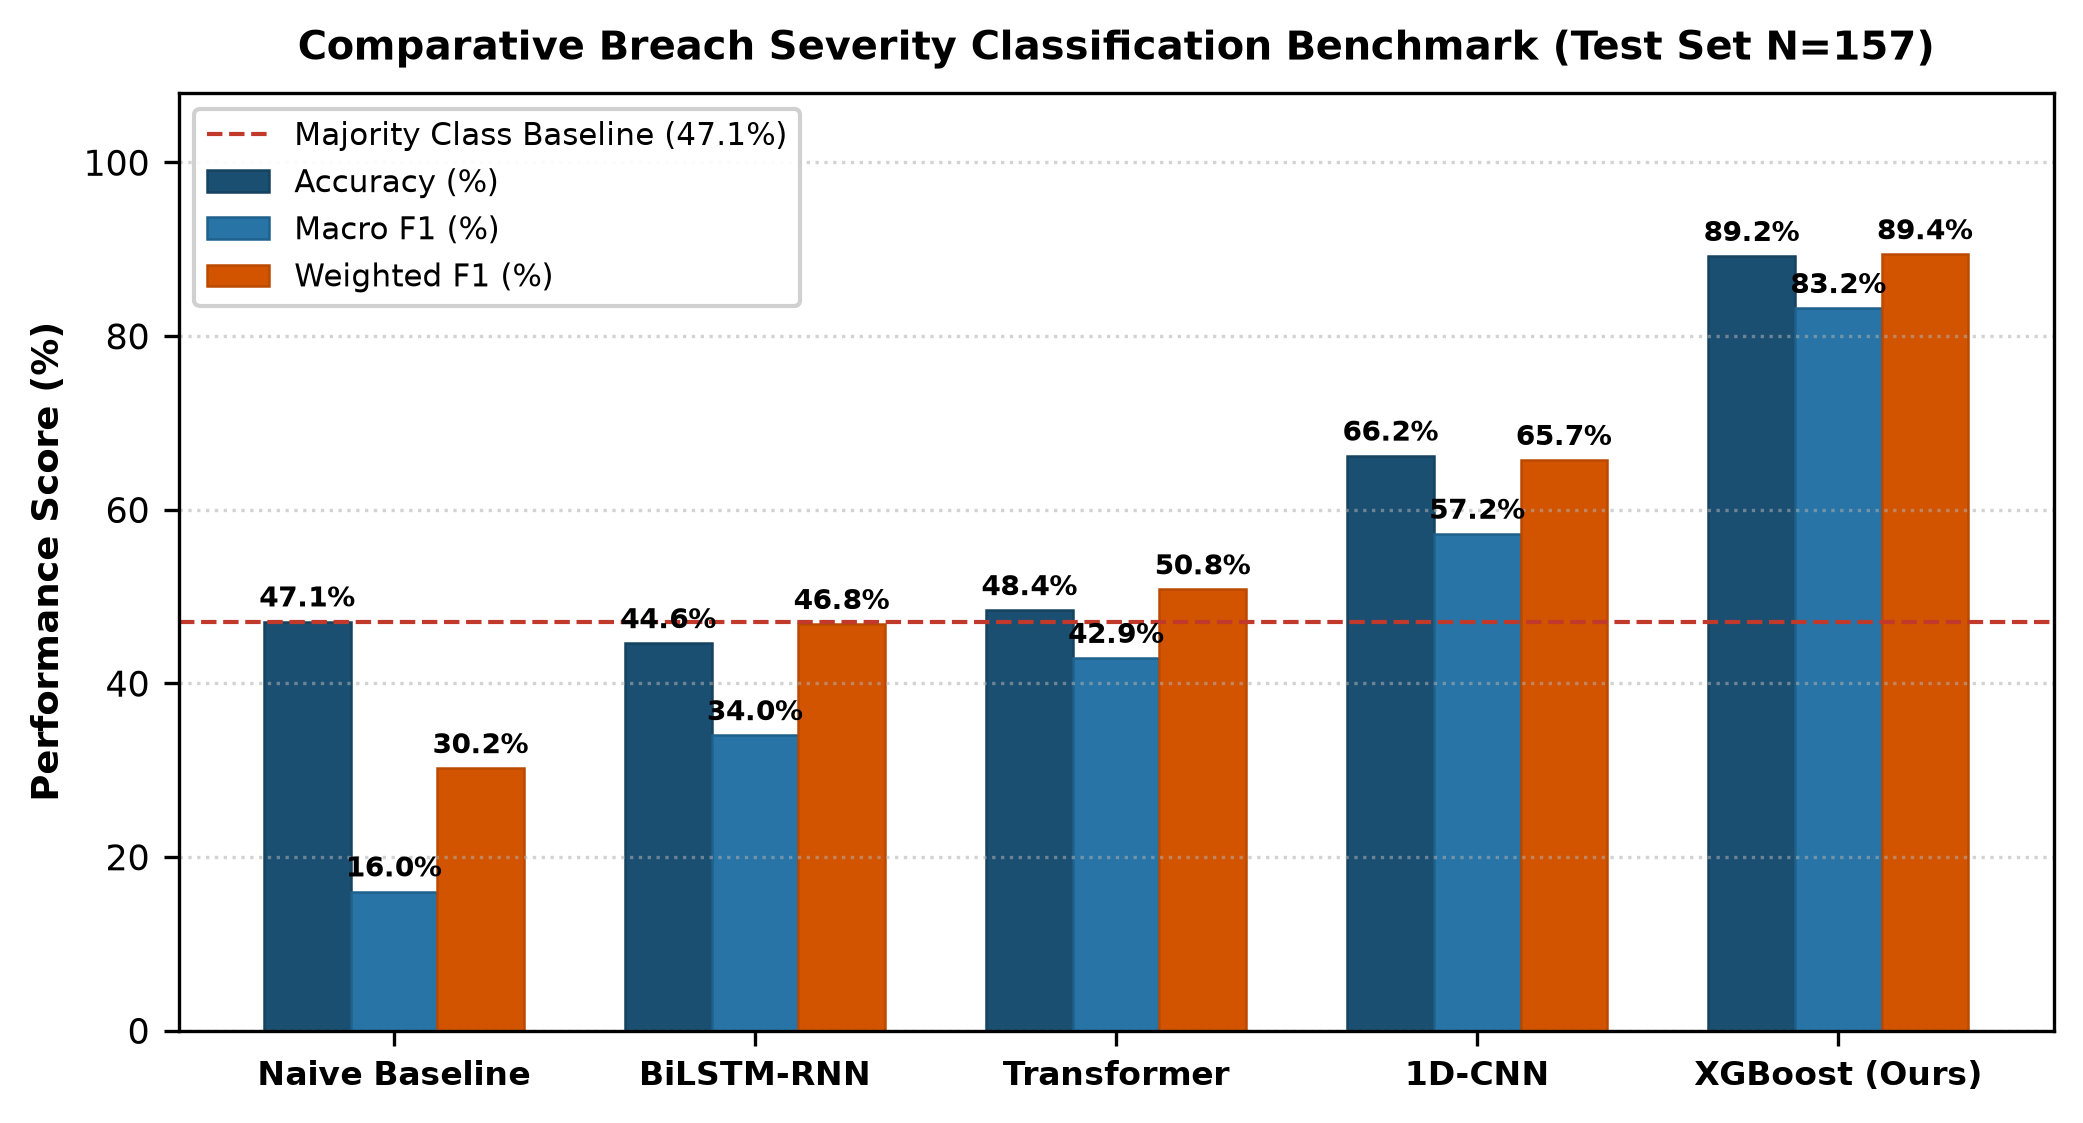
\includegraphics[width=0.98\columnwidth]{figures/fig_model_comparison.png}
\caption{Comparative severity classification benchmark across models on held-out test set ($N=157$).}
\label{fig:model_comp}
\end{figure}

The gap is consistent with Grinsztajn et al.'s finding that tree-based models retain an advantage on medium-sized tabular data \cite{grinsztajn2022why}: BreachShield's DataClasses vocabulary is a sparse, unordered categorical space, for which recurrent and attention architectures impose an artificial sequential or positional bias that tree splits do not.

\begin{figure}[htbp]
\centering
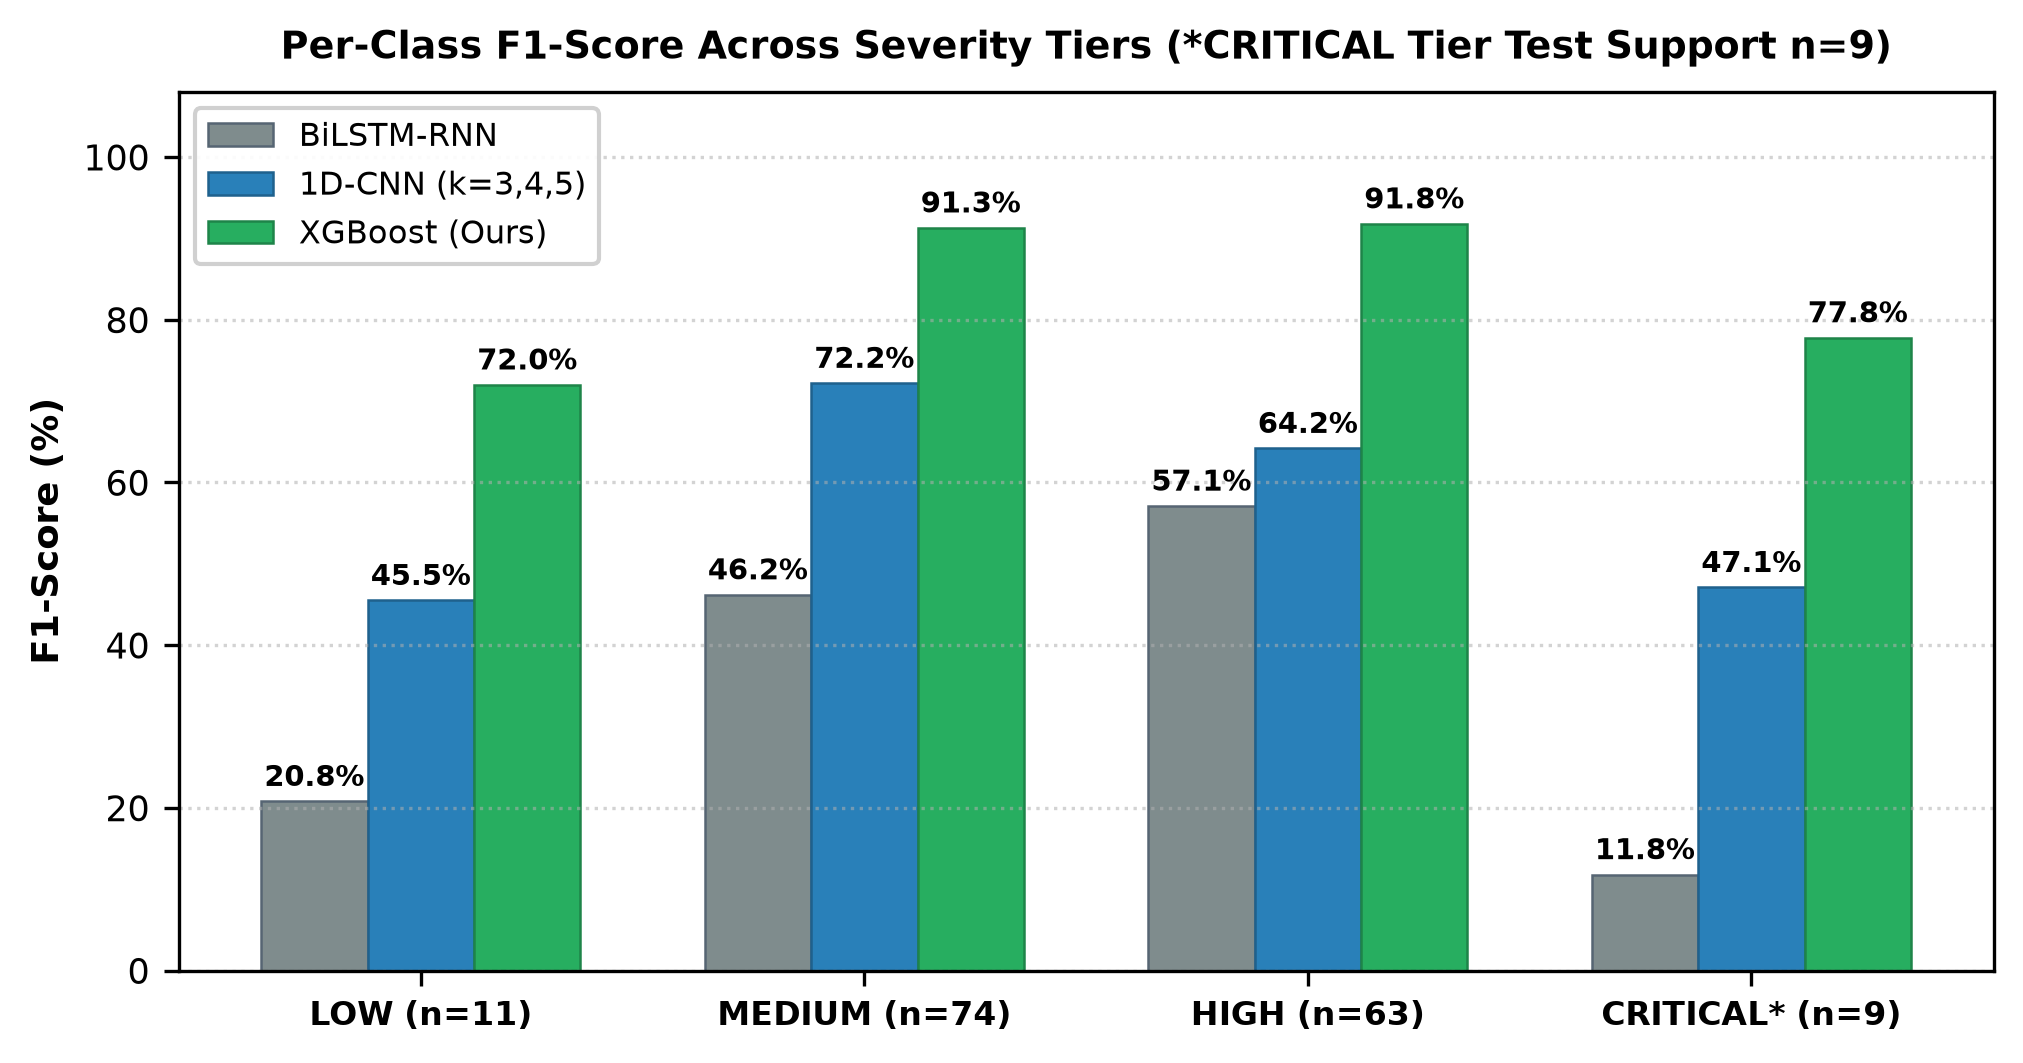
\includegraphics[width=0.98\columnwidth]{figures/fig_per_class_f1.png}
\caption{Per-class F1-score across severity tiers (*CRITICAL tier test support $n=9$).}
\label{fig:per_class}
\end{figure}

\subsection{Production Deployment Status}
Despite its strong benchmark performance, the checkpoint-loaded XGBoost severity model is not the production search-path scorer. Production risk scoring is computed by a deterministic, explainable rule-based engine (\texttt{riskEngine.js}) evaluating credential-category sensitivity, source reliability, and breach recency --- all confirmed, on direct source inspection, to be genuinely computed from record data rather than fixed constants. XGBoost is retained as a validated research artifact because live OSINT feeds do not reliably supply the complete DataClasses, volume, and verification fields the model's feature contract requires. Separately, a live pretrained URL-transformer classifier (UrlBERT) is deployed on the actual search path and confirmed functioning against a known-phishing test URL with 0.9999 confidence.

\section{Blockchain Audit Trail}
\label{sec:blockchain}
Audit events are canonicalised (sorted-key JSON) and hashed into Merkle leaves, batched by a 16-record or 60-second window, and anchored to \texttt{AnchorRegistry.sol} on a local Hardhat EVM node.

\begin{figure}[htbp]
\centering
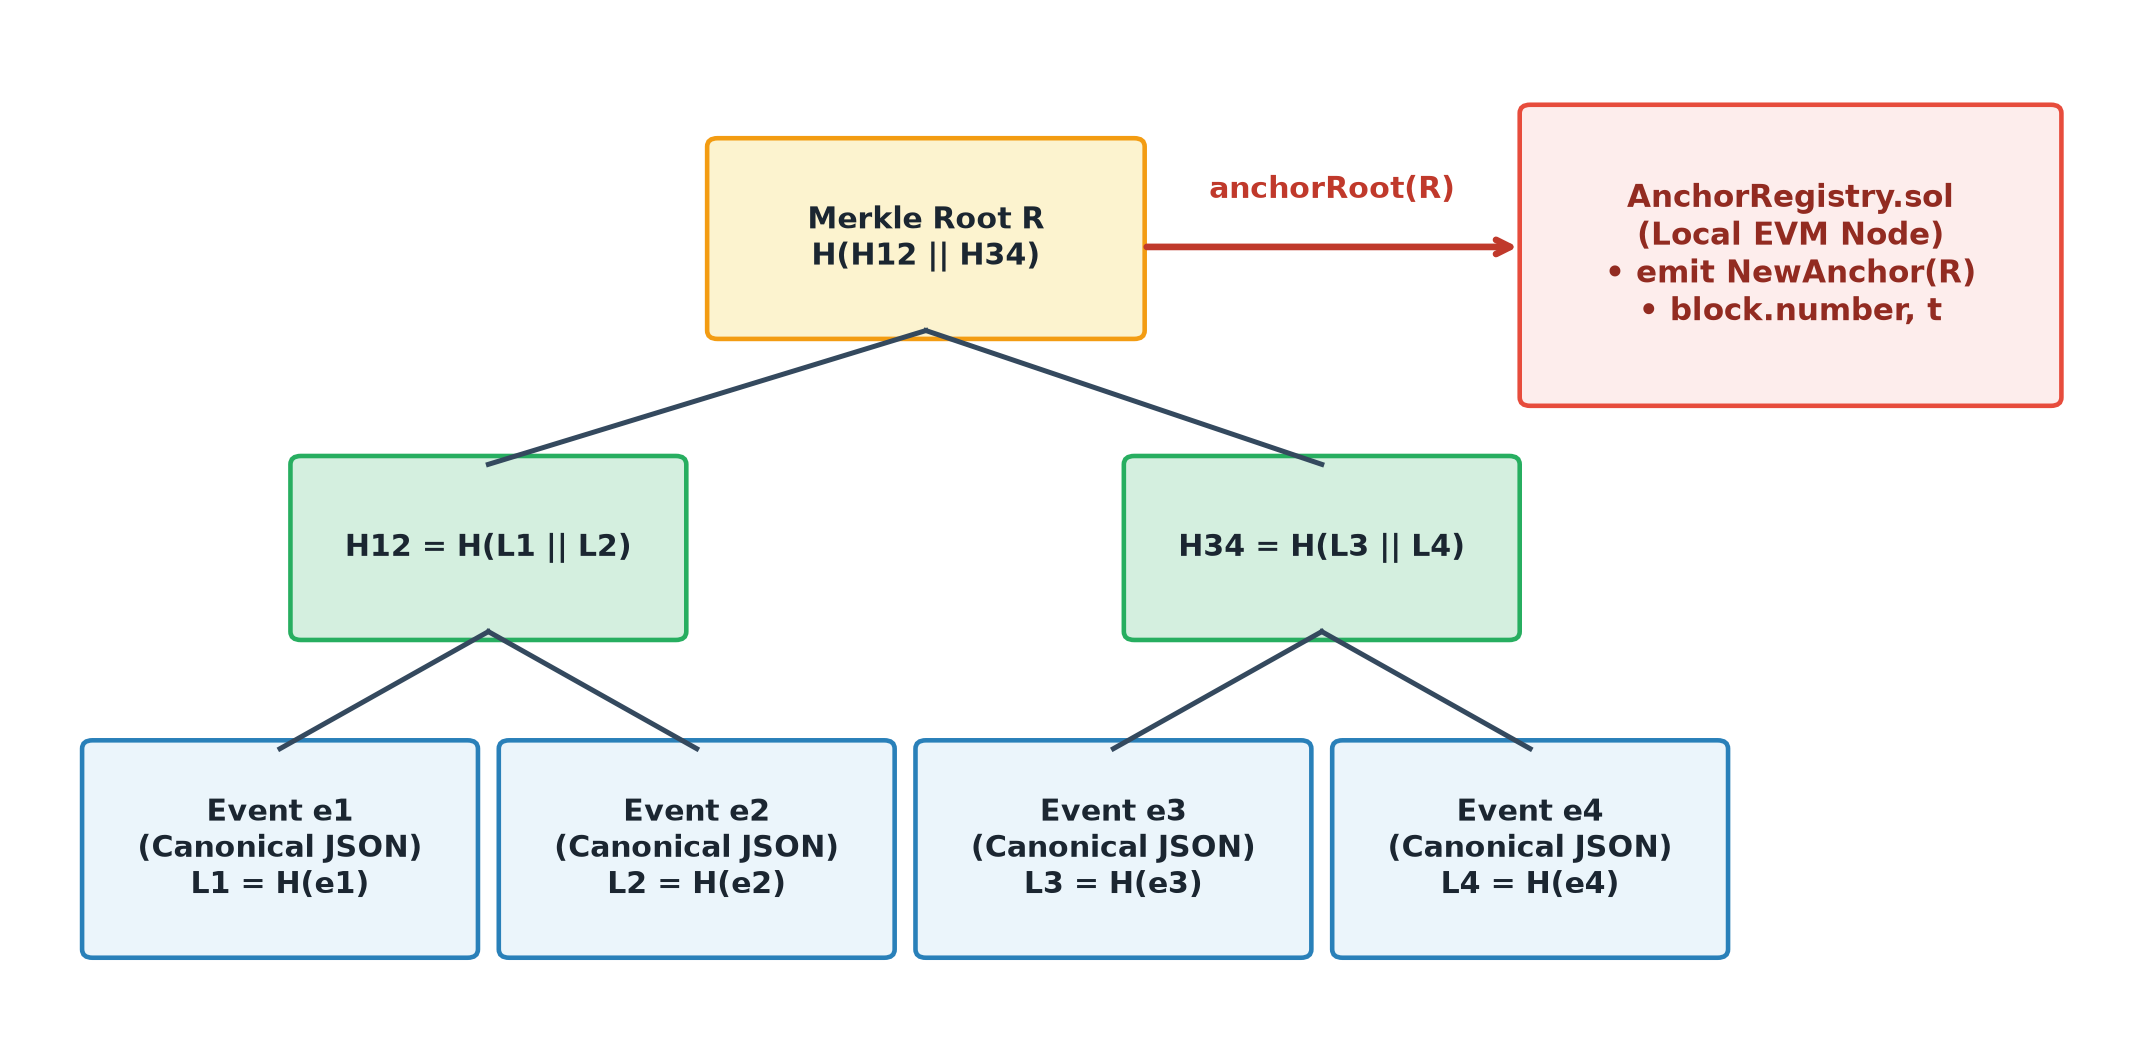
\includegraphics[width=0.98\columnwidth]{figures/fig_merkle_anchoring.png}
\caption{Merkle batching and EVM anchoring workflow (illustrative, 4-leaf batch; production batch size is 16).}
\label{fig:merkle}
\end{figure}

\subsection{Current Verified Status}
Direct testing of a clean local deploy confirms \texttt{AnchorRegistry.sol} compiles successfully.
Auto-deployment on node restart currently fails: with \texttt{ANCHOR\_PRIVATE\_KEY} unset in the local environment, Hardhat's configured account list is empty, \texttt{getSigners()} returns no deployer, and the deploy script throws at the point it attempts to read the (undefined) deployer's address. This is a configuration defect, not a design flaw in the batching or anchoring logic itself, and is corrected by supplying the missing credential; we report it as currently unresolved rather than claim a verified deploy that does not presently succeed.

\section{Three-Stage Empirical Verification Methodology}
\label{sec:verification}
Because significant portions of BreachShield were built with AI coding-agent assistance, the team adopted a policy that no capability claim would be retained in project reporting without independent, live re-verification, executed in three stages.

\begin{figure}[htbp]
\centering
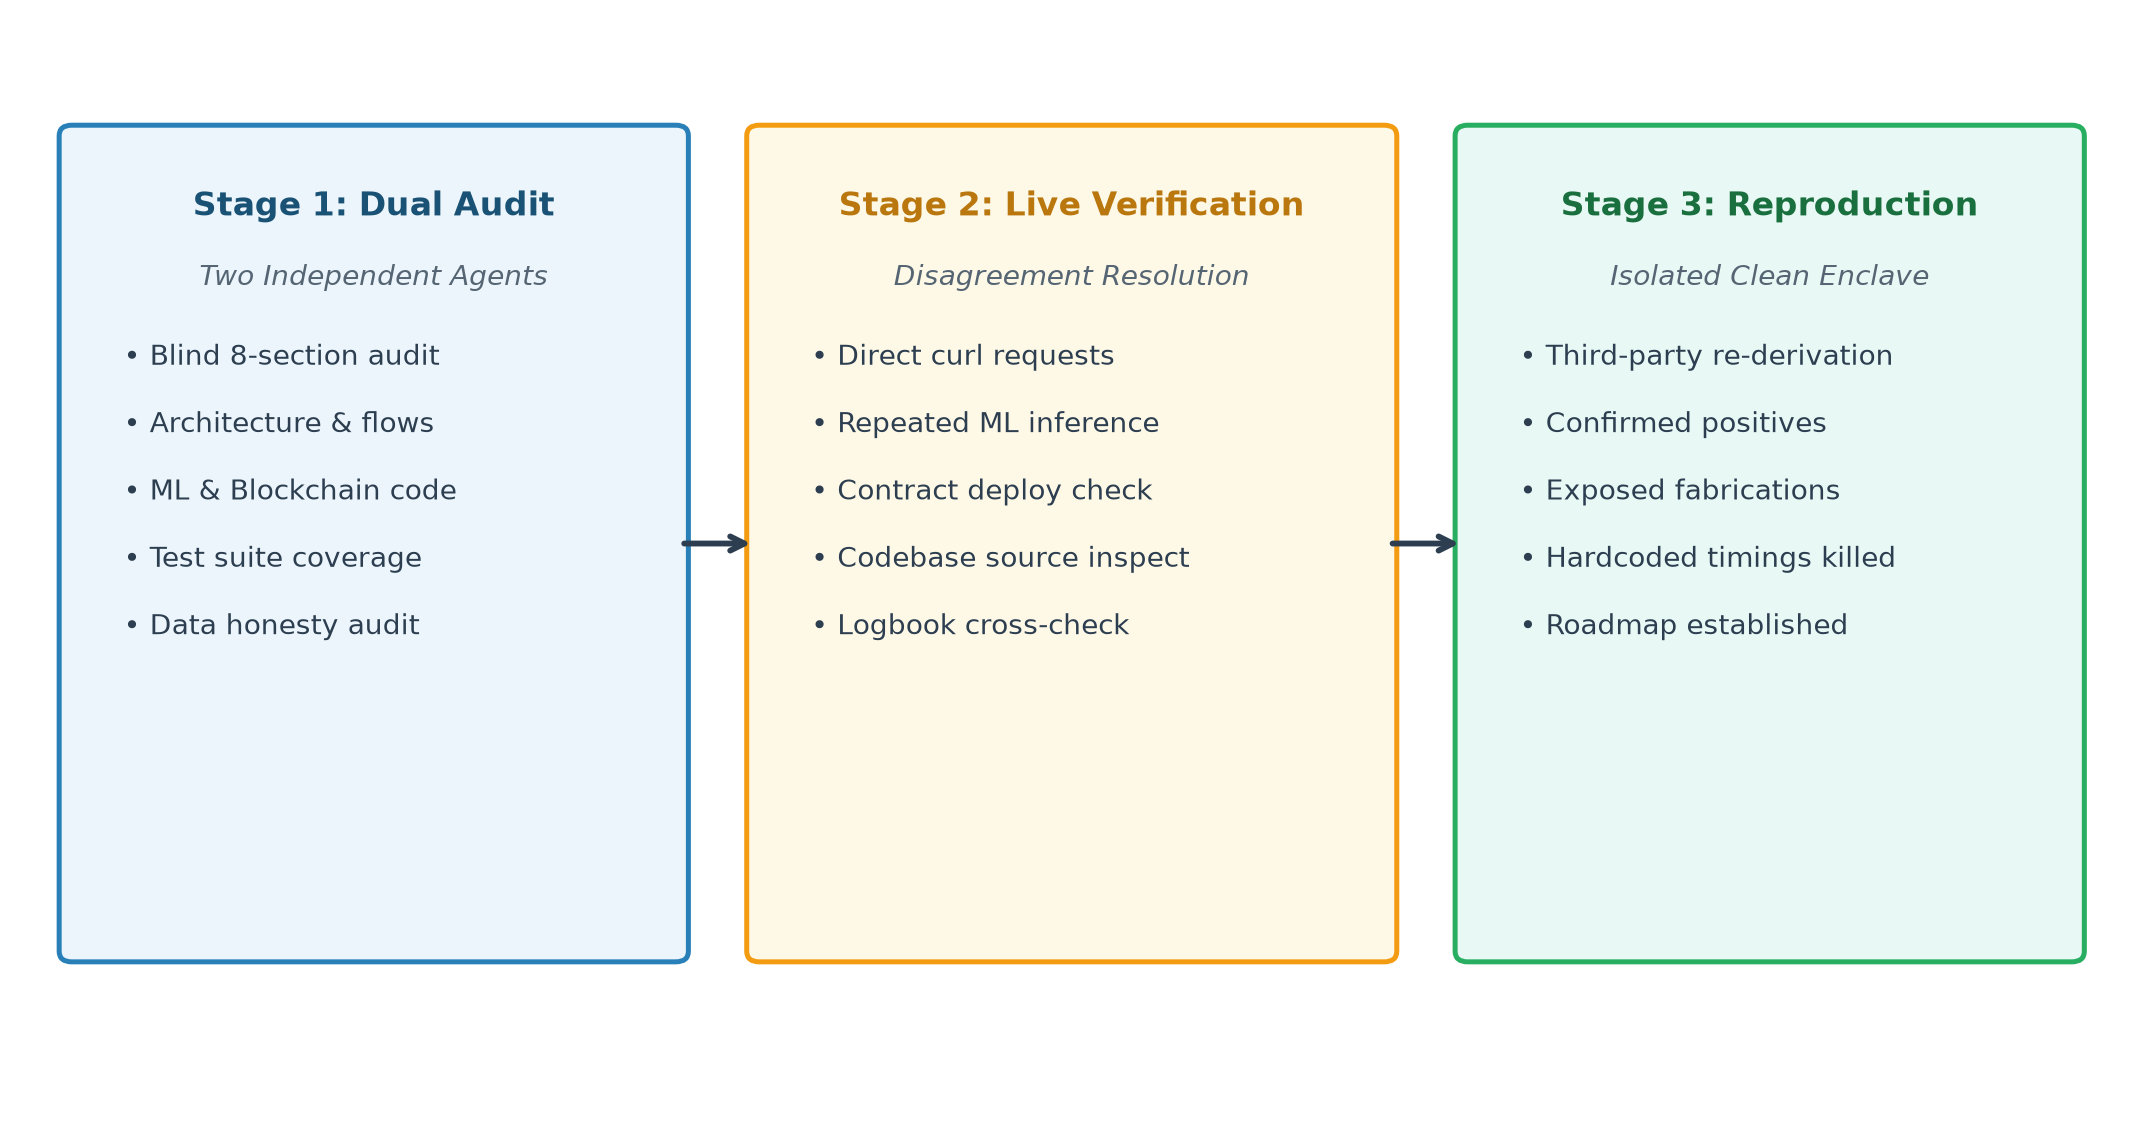
\includegraphics[width=0.98\columnwidth]{figures/fig_verification_methodology.png}
\caption{Three-stage empirical verification methodology funnel: Dual Audit $\to$ Live Cross-Checking $\to$ Reproduction.}
\label{fig:funnel}
\end{figure}

\textbf{Stage 1 --- Dual independent audit.} Two separately-prompted AI audit agents, without access to each other's output, each performed an eight-section review of the codebase (architecture, data flow, ML pipeline, blockchain, security, testing, documentation accuracy, data-source honesty).

\textbf{Stage 2 --- Live cross-checking.} Disagreements between the two audits were resolved by running direct, live commands against the running system --- \texttt{curl} calls to live endpoints, direct source reads, and repeated inference calls to test determinism --- rather than by adjudicating between the two reports.

\textbf{Stage 3 --- Independent third-party reproduction.} A third party, without access to either prior audit's conclusions, re-derived results from raw data and raw source in an isolated environment.

This process both confirmed genuine, previously-unverified positive results (Section~\ref{sec:results}) and surfaced specific fabricated or broken claims, including: latency figures (round-trip search latency, client-hash timing) that existed only as hardcoded strings inside paper-generation scripts and corresponded to no measurement anywhere in the codebase; and a set of literature citations, discussed in Section II's predecessor drafts, that were never independently checked before being written into early project documentation. We report this not to discredit the project but because verifying and correcting such claims before publication is, in our view, the more defensible response than omitting the finding.

\section{Results and Empirical Verification}
\label{sec:results}

\begin{table}[htbp]
\caption{Verification Summary}
\label{tab:eval}
\centering
\scriptsize
\begin{tabular}{lp{4.5cm}}
\toprule
\textbf{Claim} & \textbf{Verified status} \\
\midrule
$k$-anonymity search & Live-tested; correct prefix/bucket round trip \\
Severity classifier & 89.2\% test accuracy; checkpoint-loaded, deterministic \\
Backend test suite & 101/101 passing, 26 suites (both default and SKIP\_OTP=false) \\
Frontend test suite & 50/50 passing, 3 suites \\
Risk-scoring engine & Confirmed genuinely computed (source-inspected) \\
Live URL classifier & Confirmed functioning; 0.9999 confidence on test case \\
Merkle audit batching & Construction logic verified; contract compiles \\
Blockchain auto-deploy & Currently fails --- missing deployer credential \\
System latency benchmarks & No measurement exists; prior figures were fabricated \\
\bottomrule
\end{tabular}
\end{table}

\section{Critical Discussion}
The pattern underlying Table~\ref{tab:eval}'s unresolved items is consistent: each was a claim that satisfied the surface shape of a requirement (an endpoint exists, a number is quoted, a deploy step runs) without satisfying its substance, and none were caught by the project's own automated test suite. This is consistent with broader findings on LLM-assisted code and text generation producing plausible but unverified output. For a platform whose core value proposition is trustworthy breach reporting, this has a direct implication: an unverified claim about the platform's own behaviour is not a cosmetic defect but undermines the specific trust the platform asks users to place in it.

\section{Limitations and Threats to Validity}
\label{sec:limitations}
The $k$-anonymity search protocol uses the standard HIBP-style prefix-bucket construction without the stronger private-set-intersection guarantees Li et al. propose \cite{li2019protocols}; combined with OTP-gated access, the server can associate a query session with an authenticated identity even though it cannot determine the specific target within a returned bucket --- a deliberate accountability/privacy trade-off, not an oversight, but one that should not be understated. The CRITICAL severity class is represented by only 9 test-set records; per-class precision/recall on this tier carries correspondingly wide uncertainty, and the class-imbalance mitigation demonstrated by Alsubaei et al. \cite{alsubaei2024enhancing} (83\% $\to$ 98\% accuracy via SMOTE) is identified here as unapplied future work rather than a completed step. Blockchain anchoring currently targets a local EVM node rather than a public chain, and auto-deployment is presently blocked by a missing credential (Section~\ref{sec:blockchain}); public verifiability claims are therefore not made. No system-level latency benchmarks exist at the time of writing; per-request inference timings are available (UrlBERT approx. 14--31 ms) but should not be read as aggregate or percentile system performance claims.

\section{Future Work and Remediation Roadmap}
Immediate priorities are: supplying the missing deployment credential and re-verifying a clean blockchain auto-deploy; applying SMOTE or an equivalent resampling strategy to the CRITICAL severity tier following Alsubaei et al.'s demonstrated approach \cite{alsubaei2024enhancing}; and running a genuine, reproducible latency benchmark suite before any performance claim is made in future reporting. Medium-term work includes evaluating Li et al.'s private-set-intersection protocols \cite{li2019protocols} as a replacement for the current OTP-gated prefix design, and assessing public-chain anchoring following the batching pattern of Arabnouri et al. \cite{arabnouri2024secure} once local verification is complete.

\section{Conclusion}
BreachShield demonstrates a privacy-preserving breach intelligence architecture combining a $k$-anonymity search protocol, a benchmarked and reproducible ML severity classifier, and a Merkle-batched audit log, developed and verified by a final-year undergraduate team. Equally, this paper documents that AI-assisted development of the same codebase introduced specific, fabricated or non-functional claims --- concerning an unrelated model population, blockchain deployment status, and unmeasured performance figures --- that a three-stage, live-verification methodology was able to identify and correct prior to publication. We offer that methodology, alongside the verified system itself, as this paper's contribution.

\section*{Acknowledgment}
The authors thank Prof. Sushma T. M. for guidance throughout Project Phase II (Course Code: BIS786).

\bibliographystyle{IEEEtran}
\bibliography{references}

\end{document}
